%!TEX root = ../prace.tex

\section{Hlavní menu}

Po načtení hry hráč vidí hlavní menu. Denní doba i počasí se zvolí náhodně.

\begin{figure}[!ht]\centering
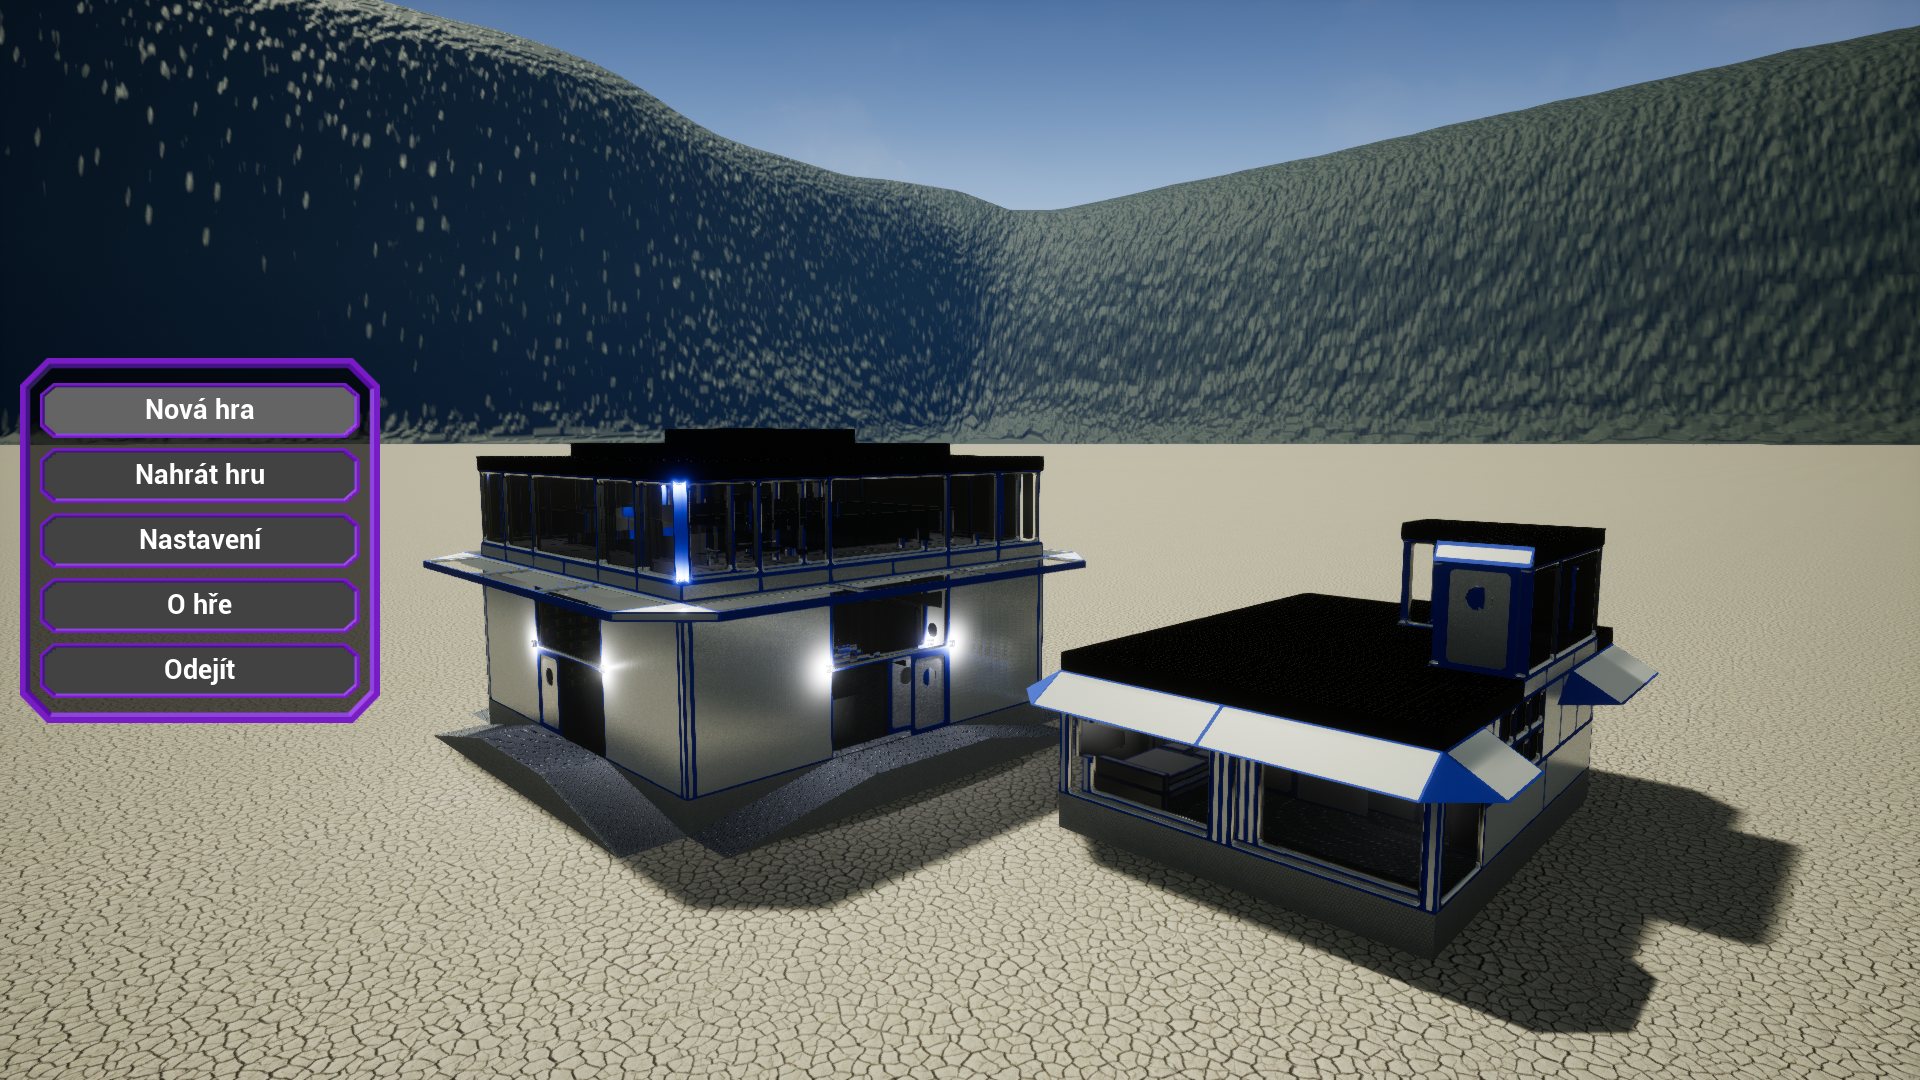
\includegraphics[ width=140mm]{../img/user/mainMenu/mmDay}

\caption{Obrazovka hlavního menu - den}
\label{fig:user_mainMenu_mmDay}

\end{figure}

\begin{figure}[!ht]\centering
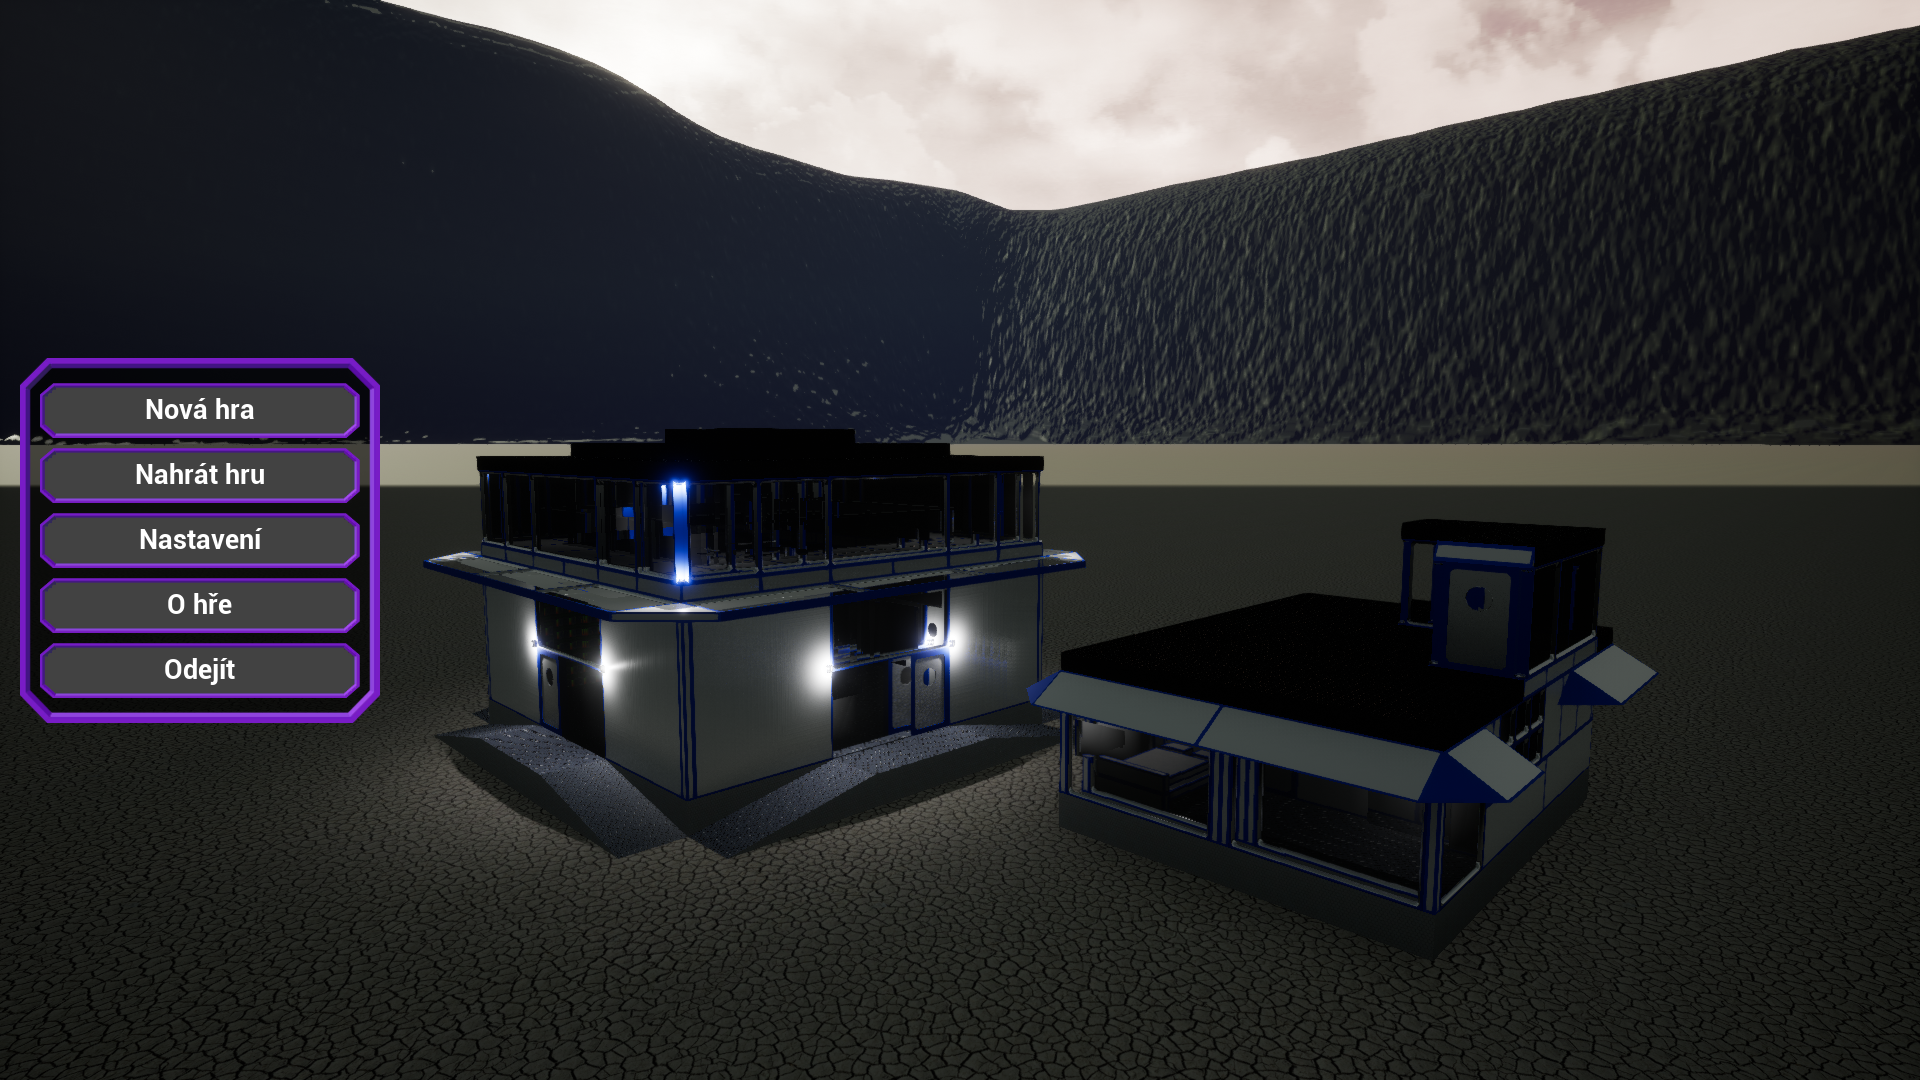
\includegraphics[ width=140mm]{../img/user/mainMenu/mmNoon}

\caption{Obrazovka hlavního menu - poledne, zataženo}
\label{fig:user_mainMenu_mmNoon}

\end{figure}

\begin{figure}[!ht]\centering
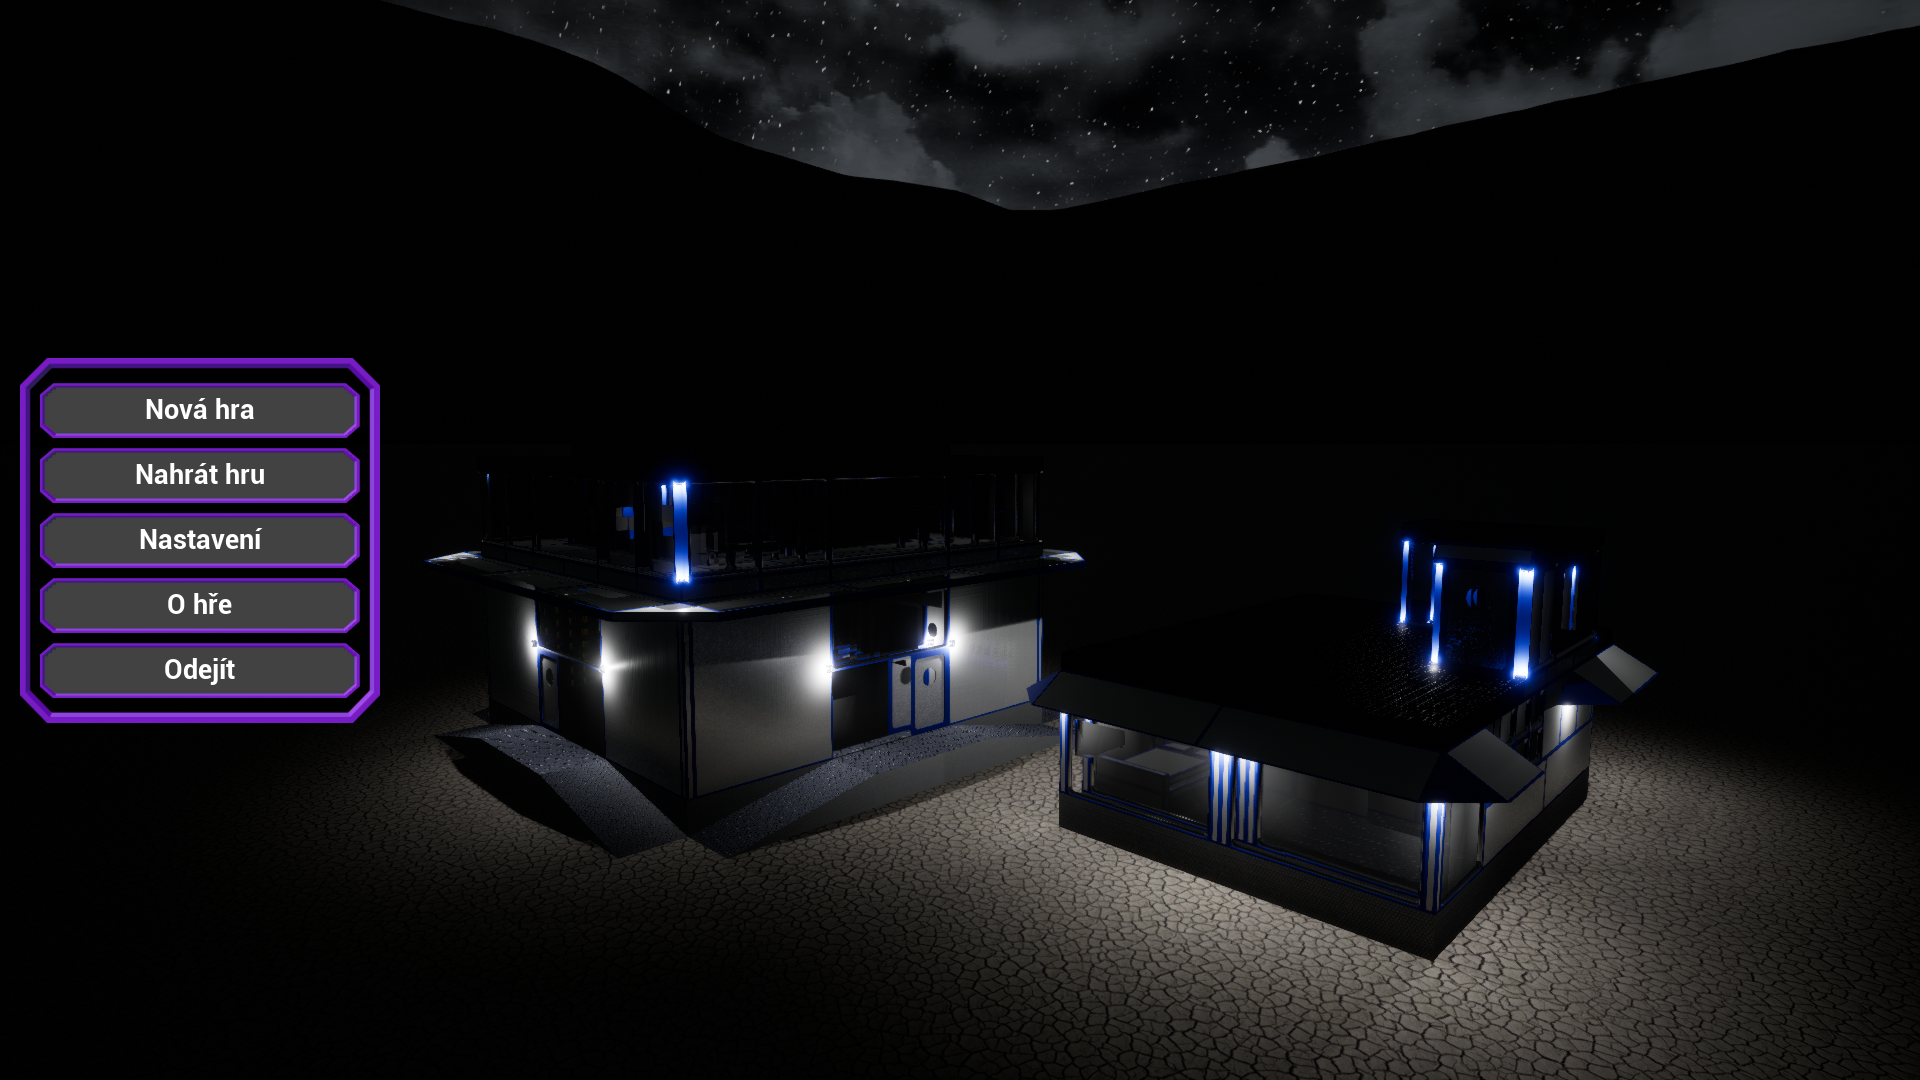
\includegraphics[ width=140mm]{../img/user/mainMenu/mmNight}

\caption{Obrazovka hlavního menu - noc}
\label{fig:user_mainMenu_mmNight}

\end{figure}



\FloatBarrier

První volba, kterou je možné zvolit, je výběr nové hry. K dispozici je několik variant s různými obtížnostmi.

\begin{figure}[!ht]\centering
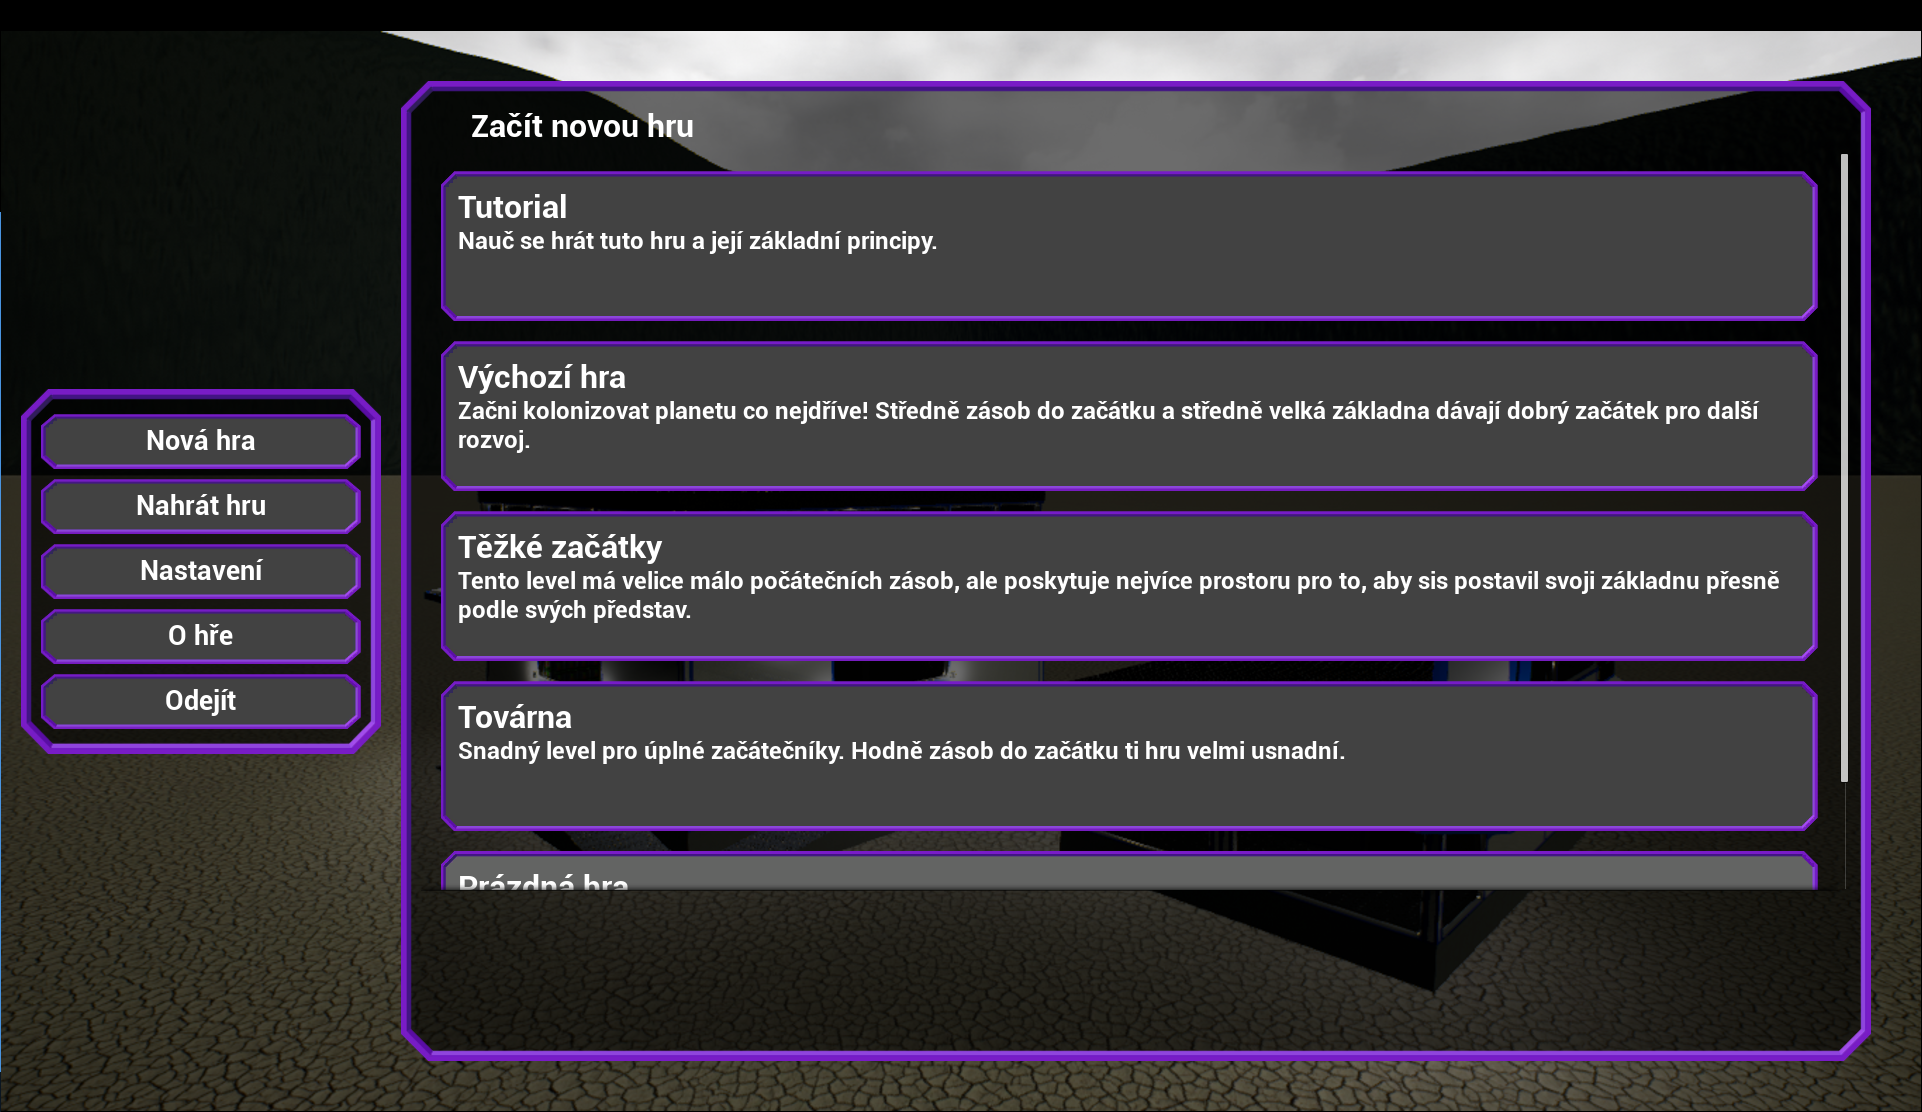
\includegraphics[ width=140mm]{../img/user/mainMenu/mmBegin}

\caption{Obrazovka hlavního menu - Nová hra}
\label{fig:user_mainMenu_mmBegin}

\end{figure}
\FloatBarrier

Pokud hráč má nějaké uložené hry, může si je nahrát kliknutím na tlačítko \textbf{Nahrát hru}. V tomto případě žádné uložené hry k načtení k dispozici nejsou.

\begin{figure}[!ht]\centering
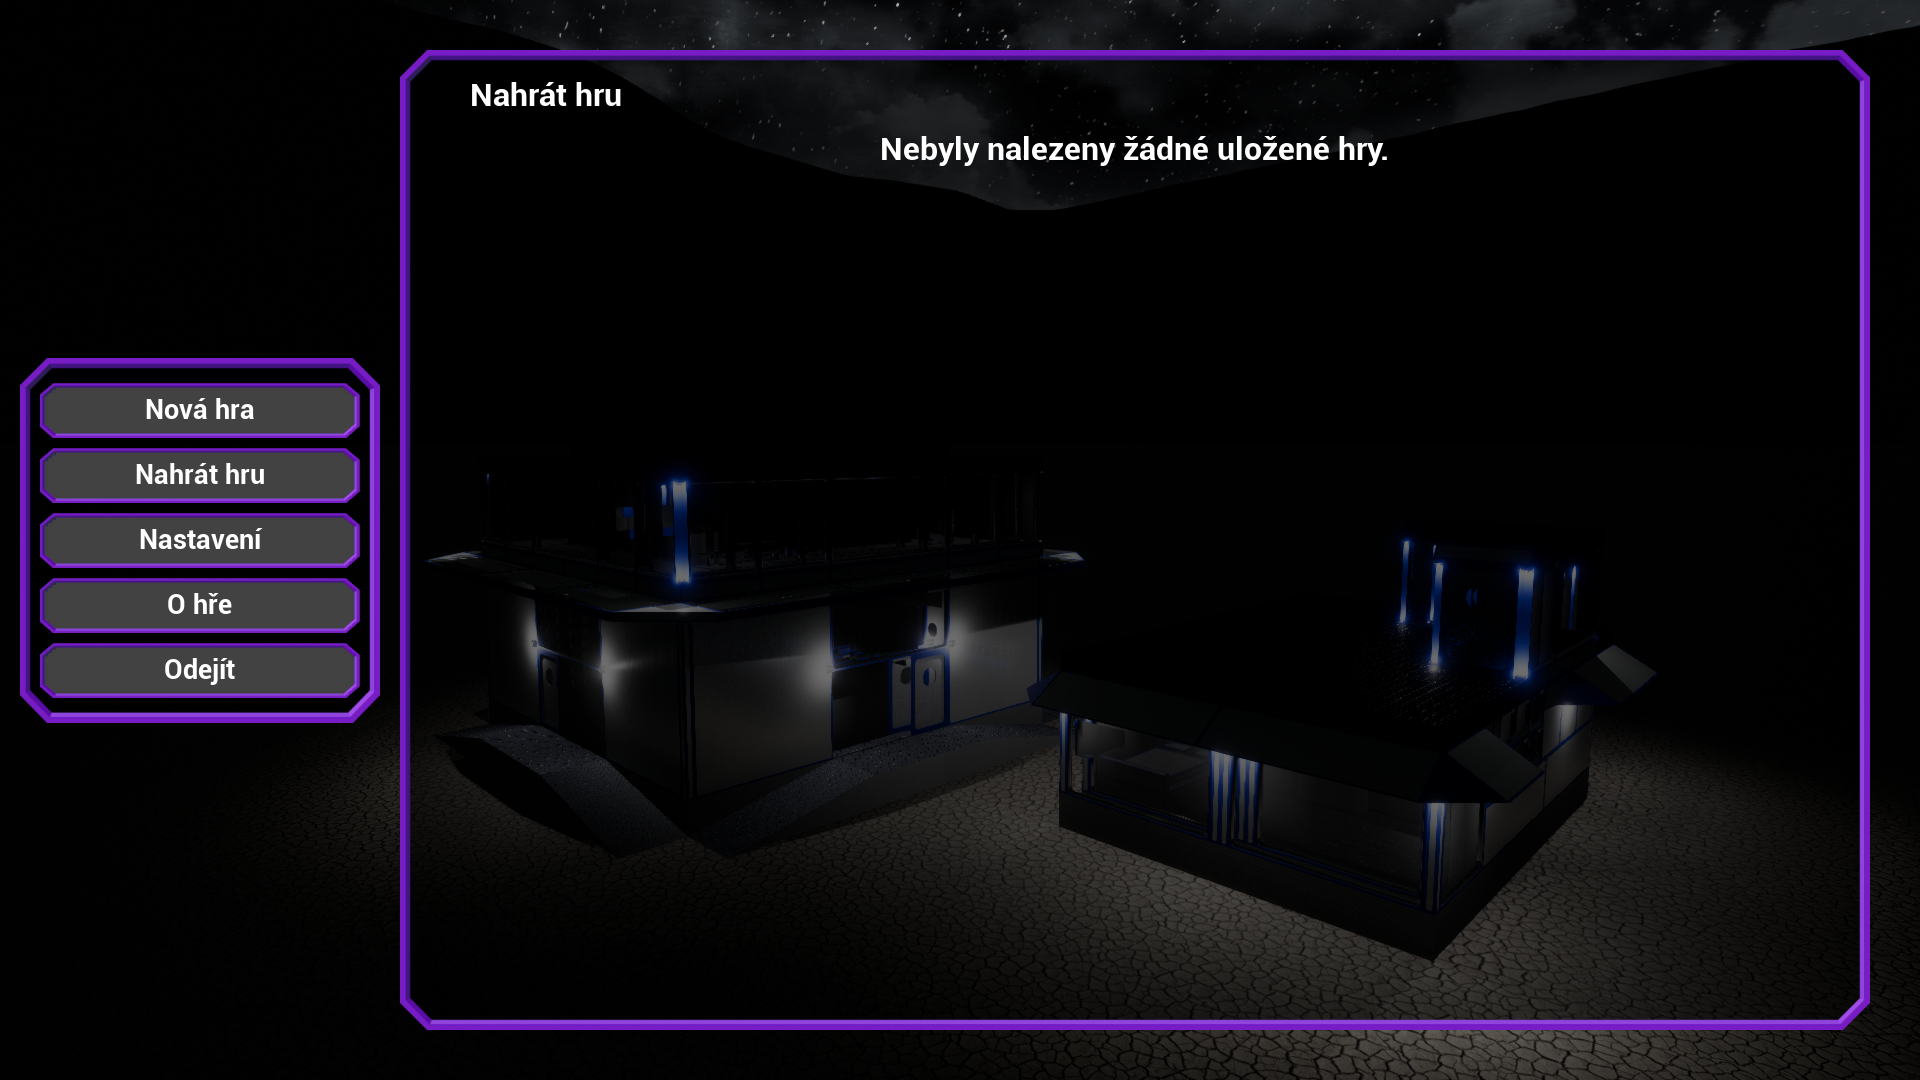
\includegraphics[ width=140mm]{../img/user/mainMenu/mmLoad}

\caption{Obrazovka hlavního menu - Nahrát hru}
\label{fig:user_mainMenu_mmLoad}

\end{figure}
\FloatBarrier

Pod položkou \textbf{Nastavení} může uživatel měnit herní, zvuková a grafická nastavení hry. Nastavení se aplikují a ukládají okamžitě, výjimkou je pouze položka \textit{Animace generátoru energie}, která se projeví až po změně levelu. V případě konfigurace z hlavní nabídky se nastavení projeví okamžitě, v případě konfigurace během rozehrané hry je potřeba vyvolat opětovné načtení uložené hry, nebo znovu spustit novou hru.

\begin{figure}[!ht]\centering
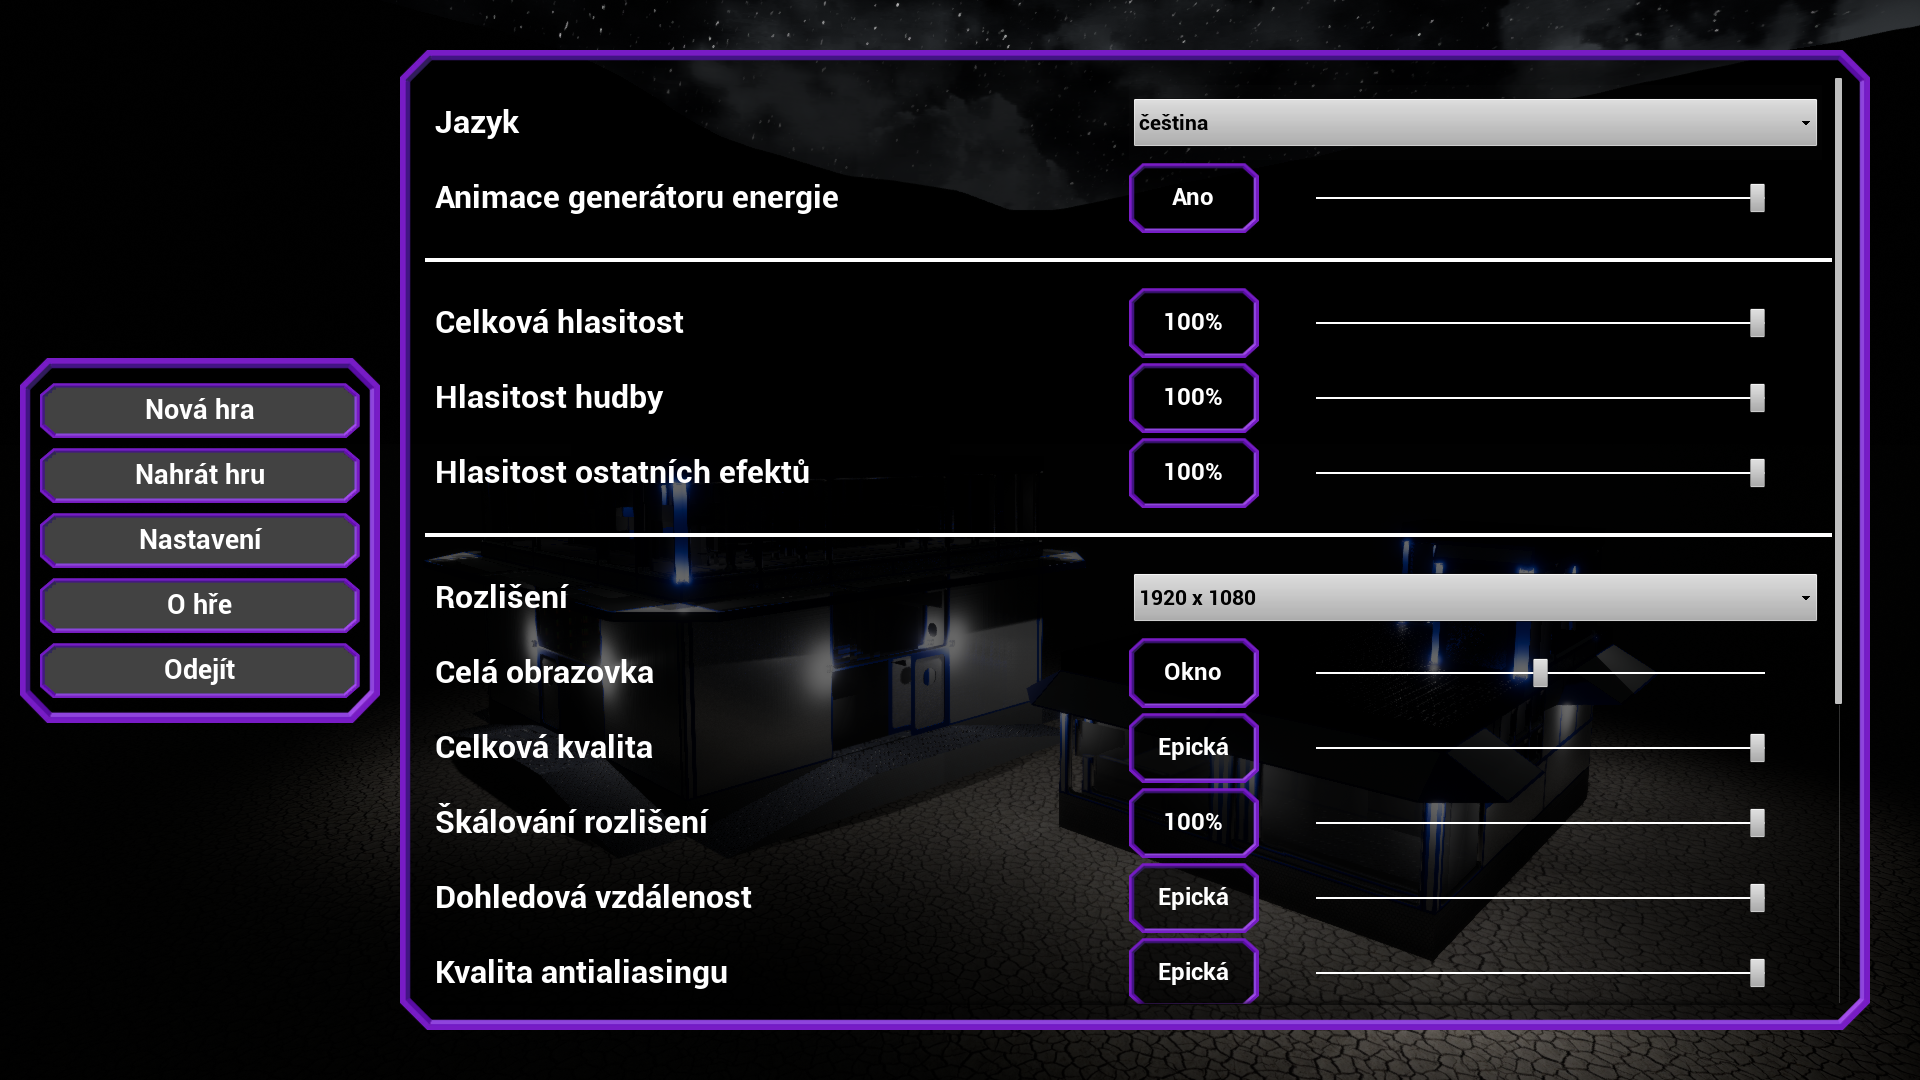
\includegraphics[ width=140mm]{../img/user/mainMenu/mmSettings}

\caption{Obrazovka hlavního menu - Nastavení}
\label{fig:user_mainMenu_mmSettings}

\end{figure}

\FloatBarrier